\begin{figure}[tbp]
	\begin{center}
		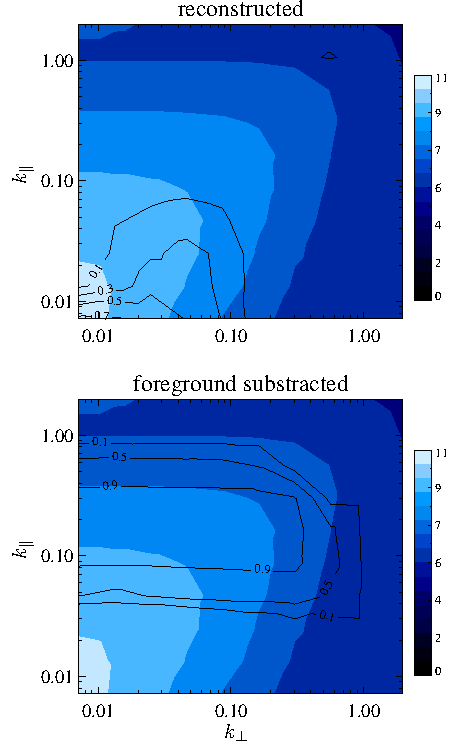
\includegraphics[width=0.48\textwidth]{vmode.pdf}
	\end{center}
	\vspace{-0.7cm}
	\caption{(Top) Contour shows the correlation $r(k_\perp,k_\parallel)$ between the real velocity field $v_z^{real}$ and $\hat v_z$ from the tidal reconstructed field; 
(Bottom) contour shows the correlation r between $v_z^{real}$ and $v_z^{fs}$ from the foreground substracted field. 
The background color indicating the level of powerspectrum of $v_z^{real}$ in logrithm, $lg(P_{v_z^{real}})$}. 
\label{fig:vmode}
\end{figure}

One of the main concerns about employing Cosmic Tidal Reconstruction is that it will import additional noise.
The question is when and why the gain will worth the loss.

To demonstrate the gain and loss, we calculate the velocity field $v_{fs}$
from the foreground substracted field $\delta_{fs}$, following identical procedure.
In Fig.\ref{fig:vmode}, contours in upper panel show the 
correlation $r(k_\perp,k_\parallel)$ between the real velocity field $v_z^{real}$ and $v_z^{fs}$; 
contours in lower panel show the
correlation r between $v_z^{real}$ and $\hat v_z$. The background color indicating the level of powerspectrum of $v_z^{real}$. 

As we can see, although importing large noise to large k modes, 
the tidal reconstruction procedure retrieve small k modes that corresponds to larger $|v(k)|$. This part of signals play a more important role in kSZ signals.
Moreover, if we calculate kSZ signal with the foreground substracted field, its correlation coefficient r with the original signal will remain 0 until $l\sim1000$.

To better understand the behavior of kSZ signal, we write Eq.(\ref{eq:ksz}) in Fourier space.\begin{eqnarray}
\Theta(\bm{k_\perp})\equiv \Theta(k_x,k_y,0)=\int d^3k \delta(\bm{k}) v_z(\bm{k_\perp}-\bm{k})\,
\end{eqnarray}

Since $v(\bm{k})\propto \delta(\bm{k})\frac{k_z}{k^2}$, 
its amplitudes drops much faster than $\delta(\bm{k})$ when k gets larger, 
therefore could be consider as delta function. So $\Theta(\bm{k_\perp})\sim\delta(\bm{k_\perp})$

However, as the foreground contaminate the small k modes, we lose the original peak in $v(k)$ and hence select different part of $\delta$ in mock kSZ signal.

On the other hand, when we perform the Tidal Reconstruction, we retrieve the modes with small $k_z$ and tolerable $k_\perp$, 
which is close to the original peak in $v(k)$ and therefore enable us to get correlated signals.

However, we have to noitice that by performing Tidal Reconstruction, 
we lost parts of small $k_\parallel$ modes(discussed in \cite{2015:zhu}), 
which explains why we do not get a better correlation.

Judging from Fig.\ref{fig:vmode} and previous statement, 
we claim that in an optimal case---the foreground noise is low and removed cleanly
---we have at least half density field structure remains at $k\sim 0.02$ Mpc/h, i.e. choose $R_\parallel=60$ Mpc/h, 
it is a better choise to apply cross correlation directly using the original field.

In all, the tidal reconstruction method is not designed to help us find the optimal correlation of the two signals, 
it is more like a safe belt that enable us to find a detectable correlation even when the measurement is not optimal. 
If you have good 21cm measurements, then perform the cross correlation directly, you will be likely to get good results; 
however, if measurements do not go well, with the tidal reconstruction, 
it is still feasible to perform the cross correlation, and get some trial results
---that is the value of the method.


